The main sources of input information required for a risk calculation with the OpenQuake engine are an \gls{exposure model} and a physical \gls{vulnerability model} or \gls{fragility model} (in addition to the calculation type and the region of interest). An \gls{exposure model} for a given category of asset (e.g. population, buildings, contents) describes, at each location of interest within a given region, the value of each \gls{asset} of a given \gls{taxonomy}. The physical \gls{vulnerability model} described the loss ratio distribution for a set of intensity measure levels, while the \gls{fragility model} provides the probability of exceeding a set of damage states, given a set of intensity measure levels. %_________________________________________________________
\section{Exposure}
\index{Exposure}
The OpenQuake engine requires an \gls{exposure model} that needs to be stored according to the respective Natural hazards' Risk Markup Language (NRML) schema (see \href{https://github.com/gem/oq-nrmllib}{oq-nrmllib}). More information on the formats of this input model is provided in the OpenQuake Engine User Manual. This file format can include several typologies of asset such as population or buildings. The following parameters are currently being used to describe each asset in the exposure model: 

\begin{itemize}
\item Asset reference: A unique key used to identify the \gls{asset} instance;
\item Location: Geographic coordinates of the \gls{asset} expressed in decimal degrees;
\item Taxonomy: Reference to the classification scheme that describes the \gls{asset};
\item Number: A numerical value describing the number of units at the given location (e.g. building count).
\item Area: This parameter specifies the built-up area of the asset, and can be defined in the two following ways: the aggregated area (i.e. the total built-up area of all the units at a given location, with a certain \gls{taxonomy}); area per unit (i.e. the average built-up area for a single building);
\item Structural cost: This parameter represents the structural replacement cost of the \gls{asset}. This value can be defined in three possible ways: the aggregated structural cost (i.e. the total economic value of all the units with a certain \gls{taxonomy} at a given location); the cost per unit (i.e. the average value for a single building); the cost per unit of area. Further information about how the structural cost is handled within the OpenQuake engine can be found in the OpenQuake Engine User Manual.
\item Non-structural cost: This parameter is used to define the cost of the non-structural components. This cost defined in the same way as the structural cost.
\item Contents cost: This parameter is used to define the contents cost, and it can be defined in the same way as the structural cost.
\item Retrofitting cost: This parameter is used to define the economic structural cost due to the implementation of a retrofitting/strengthening intervention. The retrofitting cost can be defined in the same way as the structural cost.
\item Occupants: This parameter defines the number of people that might exist inside of a given structure. Different values of occupants can be stored according to the time of the day (e.g day, night, transit).  
\item Deductible: This parameter is used in the computation of the \gls{insuredLosses}, and it establishes the economic value that needs to be deducted from the \gls{groundupLosses}. A \gls{deductible} needs to be defined for each cost type (structural, non-structural and contents). This threshold can be defined in two ways: 1) the direct (absolute) value that will be deducted; 2) the fraction (relative) of the total cost that will be deducted. 
\item Limit: This parameter establishes the maximum economic amount that can be insured, and it also needs to be defined for each cost type. The limit can also be defined as an absolute or relative quantity.  
\end{itemize}


\section{Physical Vulnerability}
\index{Physical Vulnerability}
Physical vulnerability is defined as the probabilistic distribution of loss, given an intensity measure level. These \glspl{vulnerability function} can be derived directly, usually through empirical methods where the losses from past events at given locations are related to the levels of intensity of ground motion at those locations, or they can be derived by combining \glspl{fragility function} and \glspl{consequence function}. \Glspl{fragility function} describe the probability of exceeding a set of limit states, given an intensity measure level; limit states describe the limits to performance levels, such as damage or injury levels. \Glspl{fragility function} can be derived by expert-opinion, empirically (using observed data), or analytically, by explicitly modeling the behavior of a given asset typology when subjected to increasing levels of ground motion. \Glspl{consequence function} describe the probability distribution of loss, given a performance level and are generally derived empirically. 

Version 1.0 of the OpenQuake engine only supports physical vulnerability through the aforementioned \glspl{vulnerability function}. As part of the plans for a risk modelling toolkit, calculators are envisaged that will combine \glspl{fragility function} and \glspl{consequence function} to produce \glspl{vulnerability function} that can be input into the engine. 

\subsection{Vulnerability Functions}
\subsubsection{Discrete Vulnerability Functions}
\index{Physical Vulnerability!Discrete Functions}
In the current version of the OpenQuake engine (v1.0) discrete \glspl{vulnerability function} are used to directly estimate fatalities and economic losses due to physical damage. Discrete \glspl{vulnerability function} are described by a list of intensity measure levels and corresponding mean loss ratios (the ratio of mean loss to exposed value), associated coefficients of variation and probability distributions. The uncertainty on the loss ratio can follow a lognormal or Beta distribution. Figure \ref{fig:VFDiscrete} illustrates a discrete \gls{vulnerability function}.

\begin{figure}[ht]
\centering
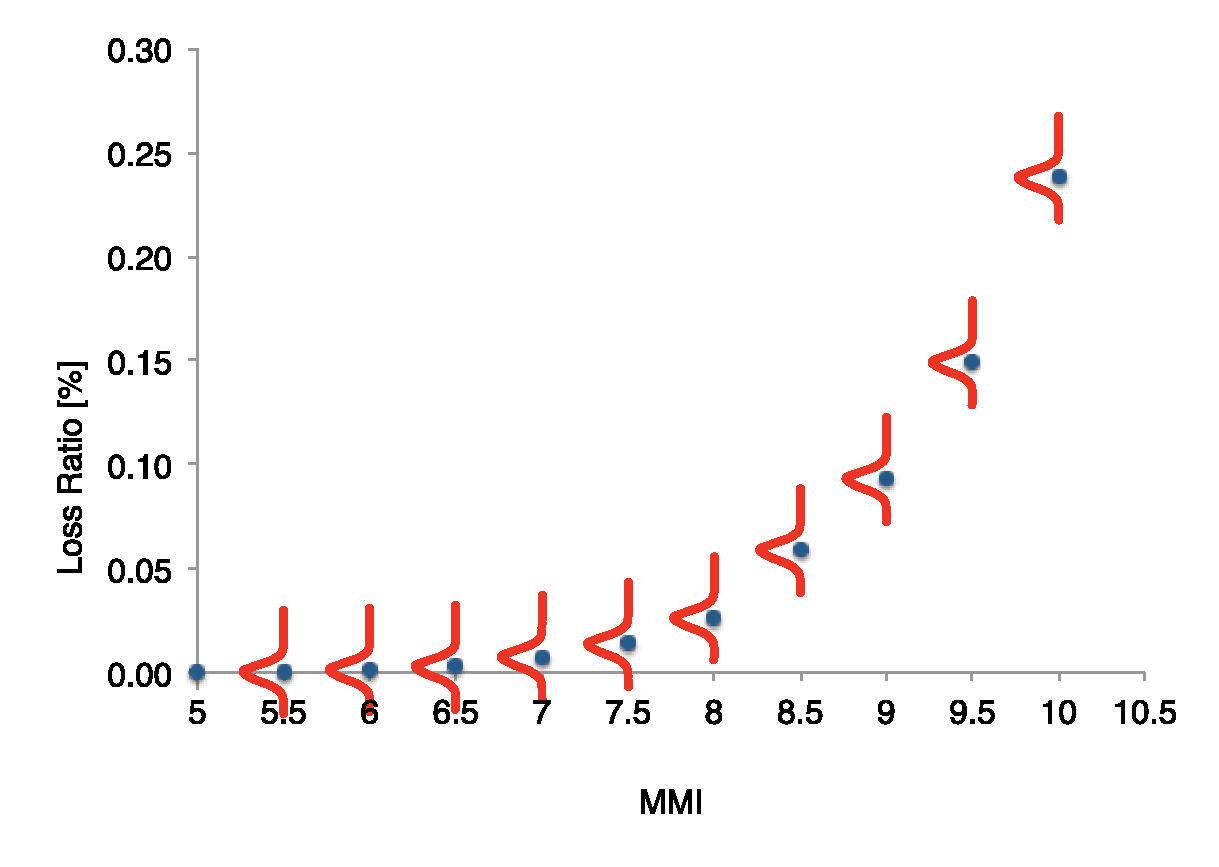
\includegraphics[width=10cm,height=6cm]{./figures/risk/VFDiscrete.eps}
\caption{Discrete vulnerability function.}
\label{fig:VFDiscrete}
\end{figure}

\color{blue}
\subsubsection{Continuous Vulnerability Functions}
\index{Physical Vulnerability!Continuous Functions}
\marginpar{Continuous vulnerability functions are not currently supported}
Continuous \glspl{vulnerability function} may be implemented in future versions of the OpenQuake engine. Continuous \glspl{vulnerability function} will probably be described by continuous distributions of mean loss ratio and other fractiles of loss ratio, with ground motion intensity. Figure \ref{fig:VFContinuous} illustrates this type of function, showing the distribution of mean loss and the 10 percent and 90 percent fractiles.

\begin{figure}[ht]
\centering
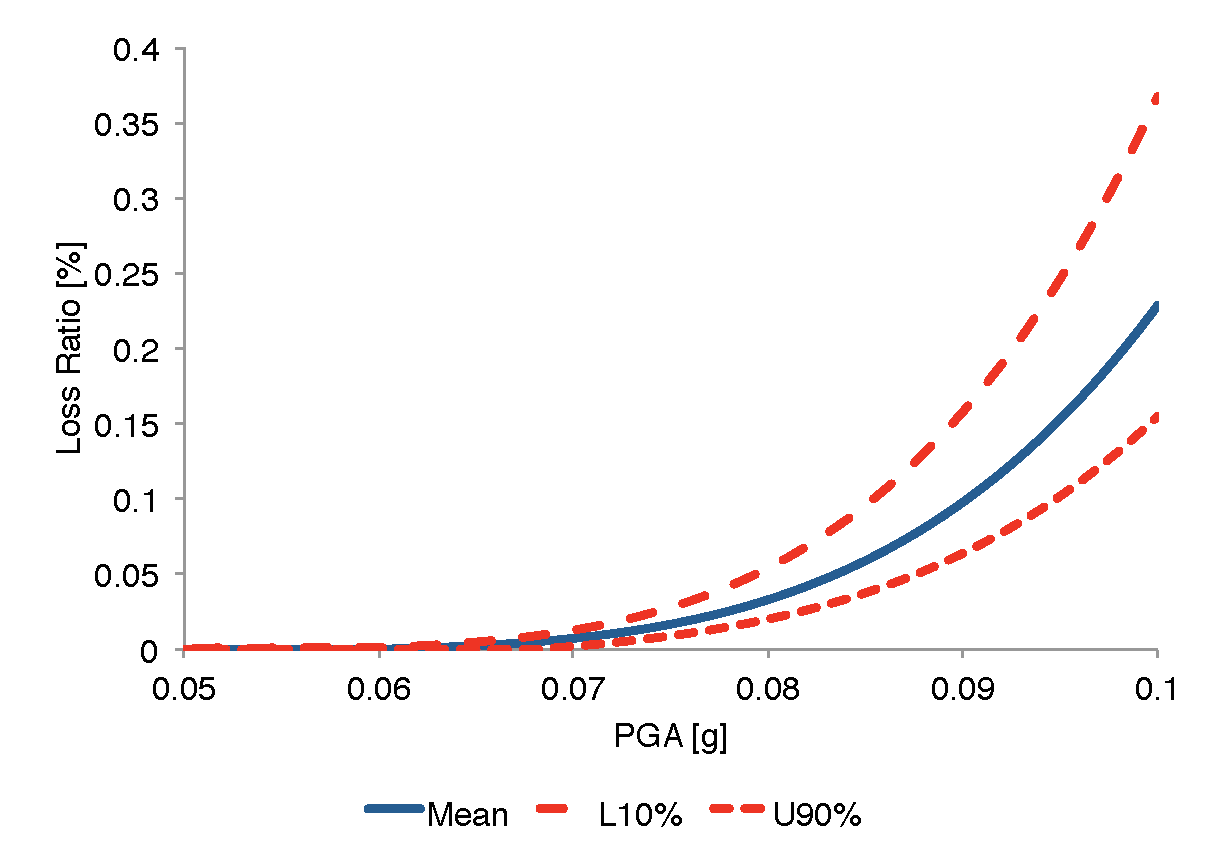
\includegraphics[width=10cm,height=6cm]{./figures/risk/VFContinuous}
\caption{Continuous vulnerability function.}
\label{fig:VFContinuous}
\end{figure}
\color{black}

\subsection{Fragility Functions}
\index{Fragility}
\Glspl{fragility function} describe the probability of exceeding a set of limit states, given an intensity measure level. When the asset category concerns structures (e.g. buildings), the intensity measure can either be structure-independent or structure-dependent. The former can be calculated directly from recorded measurements of ground shaking (e.g. peak ground acceleration, peak ground velocity, spectral acceleration at a given period of vibration, or even macroseismic intensity). The latter requires information on the characteristics of the structures in order to be calculated, for example spectral acceleration at the fundamental period of vibration, or spectral displacement at the limit state period of vibration. The calculation of these structural characteristics might be through a simple formulae (e.g. a yield period-height equation, see e.g. \citet{CrowleyPinho2004} ) or through so-called non-linear static methods, which are needed when the intensity measure is a non-linear response quantity such as spectral displacement at the limit state period of vibration (see e.g. \citet{FEMA440ATC2005}). The oq-risklib currently does not support non-linear static methods.

\subsubsection{Discrete Fragility Functions}
\index{Fragility!Discrete Functions}
\Glspl{fragility function} can be defined in a discrete way by providing, for each limit state, a list of intensity measure levels and respective probabilities of exceedance. Figure \ref{fig:FFDiscrete} presents a set of discrete \glspl{fragility function} using a macroseismic intensity measure. 

\begin{figure}[ht]
\centering
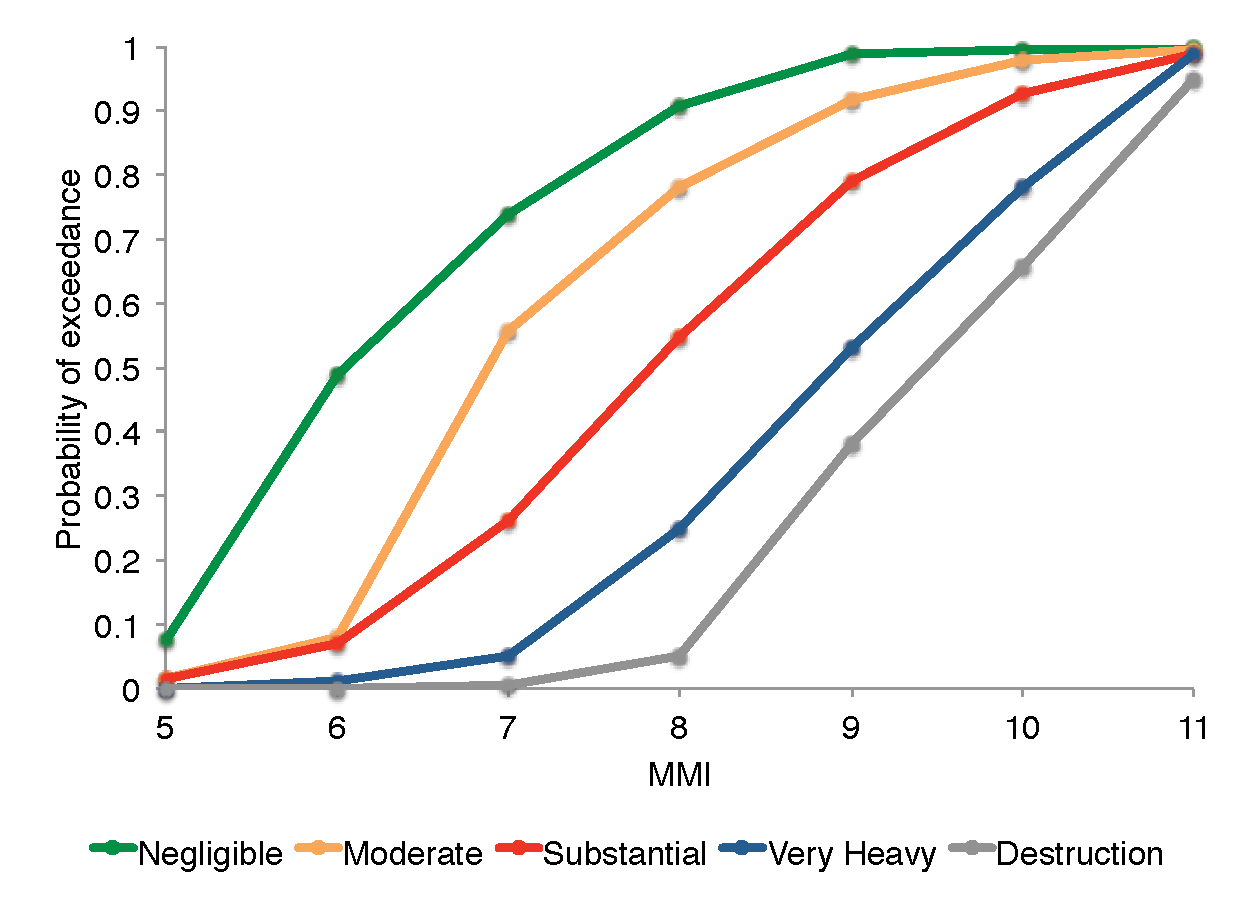
\includegraphics[width=10cm,height=6cm]{./figures/risk/FFDiscrete.eps}
\caption{Set of discrete fragility functions.}
\label{fig:FFDiscrete}
\end{figure}

\subsubsection{Continuous Fragility Functions}
\index{Fragility!Continuous Functions}
Continuous \glspl{fragility function} are defined by the parameters of a cumulative distribution function. In Figure \ref{fig:FFcontinuous} an example of a set of continuous fragility functions with a structure-dependent intensity measure is presented. 

\begin{figure}[ht]
\centering
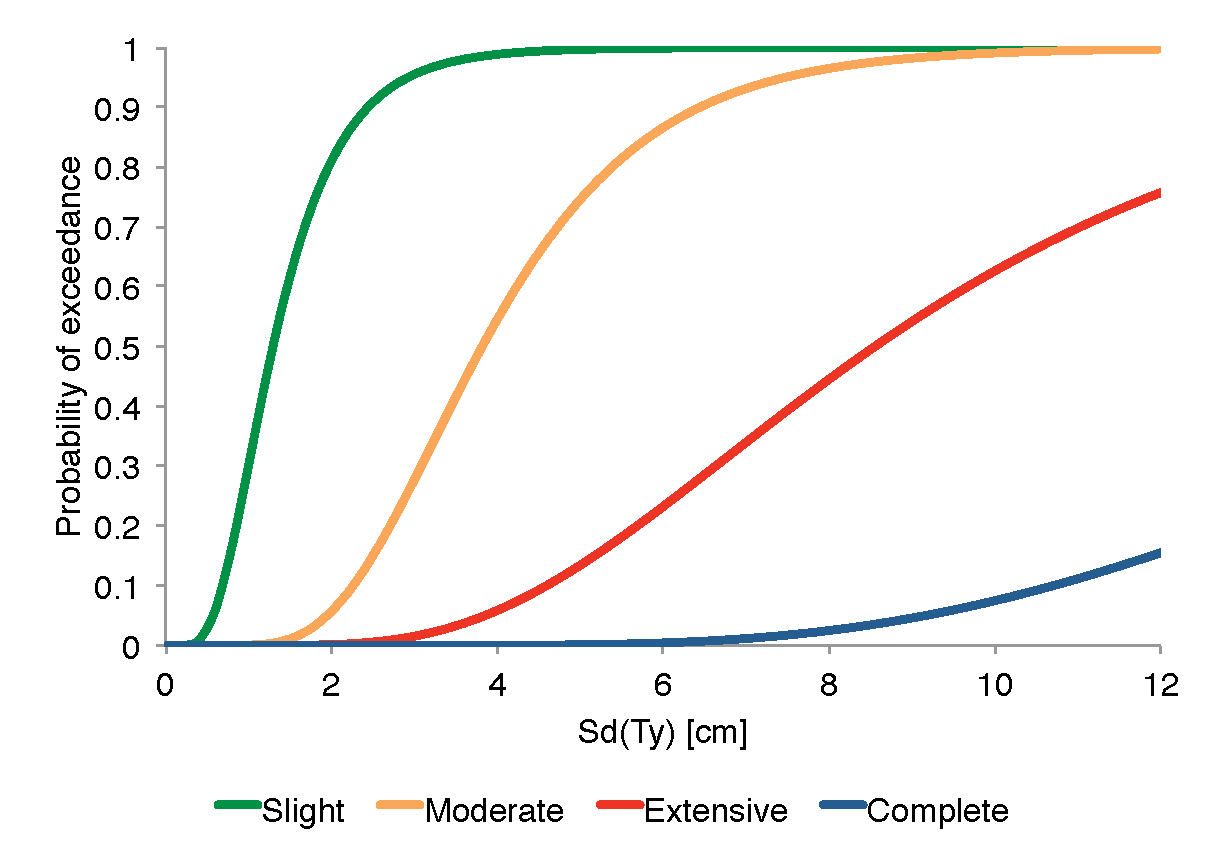
\includegraphics[width=10cm,height=6cm]{./figures/risk/FFContinuous.eps}
\caption{Set of continuous fragility functions.}
\label{fig:FFcontinuous}
\end{figure}

\color{blue}
\subsubsection{Uncertainty in Fragility Functions}
\index{Fragility!Uncertainty}
\marginpar{uncertainty in fragility functions is not currently supported}
The uncertainty in continuous \glspl{fragility function} will be accounted for in future versions of the engine. Figure \ref{fig:FF_uncertainty} shows a lognormal distribution that has been fit to the data (i.e. the fragility function), and the probabilistic distribution (i.e. mean and standard deviation) to describe the uncertainty in both the logarithmic mean and logarithmic standard deviation of the fragility function. When a set of \glspl{fragility function} for different limit states are used, it is also necessary to provide information on the correlation between the logarithmic means and logarithmic standard deviations of each limit state.

\begin{figure}[ht]
\centering
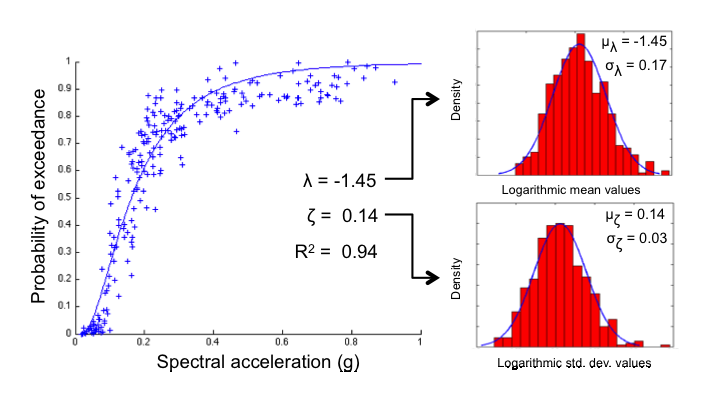
\includegraphics[width=12cm,height=6cm]{./figures/risk/FFuncertainty.eps}
\caption{Uncertainty of continuous fragility functions.}
\label{fig:FF_uncertainty}
\end{figure}


\subsection{Consequence Functions}
\index{Consequence Functions}
\marginpar{Consequence functions are not currently supported}
\Glspl{consequence function} describe the probability distribution of loss, given a performance level. For example, if the asset category is buildings and the performance level is significant damage, the \gls{consequence function} will describe the mean loss ratio, coefficient of variation and probability distribution for that level of damage. Figure \ref{fig:ConsequenceFunctions} presents the mean damage ratios for a set of performance levels proposed by two different sources. Although these functions are not directly supported, users can combine \glspl{consequence function} with \glspl{fragility function} to produce \glspl{vulnerability function} to be input into the engine.  

\begin{figure}[Ht]
\centering
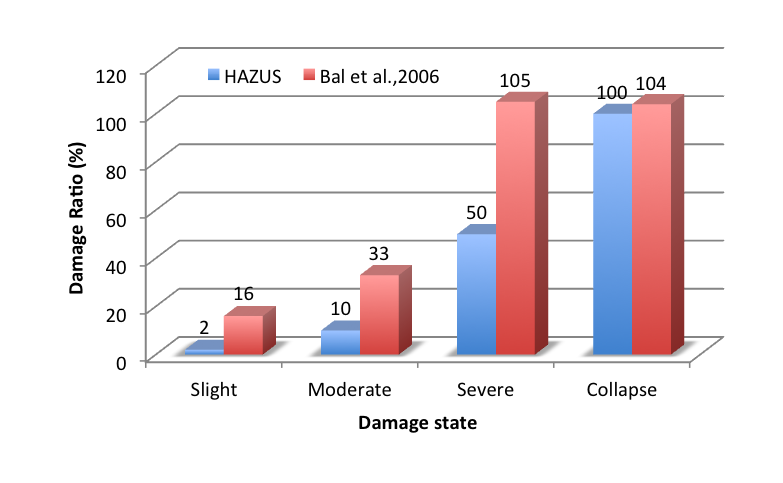
\includegraphics[width=10cm,height=6cm]{./figures/risk/ConsequenceFunction.eps}
\caption{Consequence functions adapted from  \citet{Baletal2010}}
\label{fig:ConsequenceFunctions}
\end{figure}
\color{black}
